
\documentclass{beamer}
 \usetheme[pageofpages=of,% String used between the current page and the
                         % total page count.
          alternativetitlepage=true,% Use the fancy title page.
          titlepagelogo=UlbLogos/logo-ulb,% Logo for the first page.
          watermark=,% Watermark used in every page.
          watermarkheight=25px,% Height of the watermark.
          watermarkheightmult=6,% The watermark image is 4 times bigger
                                % than watermarkheight.
          ]{Torino}

\usepackage{epstopdf}
\usepackage{spverbatim}
\usepackage{caption}
\usepackage{pgfpages}
\usepackage{hyperref}
\usepackage{tikz}

\usetikzlibrary{positioning,shadows,arrows,intersections,calc,automata}

% Nouvelle is a green and red alternative to the chameleon color theme.
\usecolortheme{nouvelle}
\logo{
\includegraphics[height=1cm]{UlbLogos/ULBPolytech.eps}}

\pgfdeclarelayer{background}
\pgfdeclarelayer{foreground}
\pgfsetlayers{background,main,foreground}
 
% Define block styles  
\tikzstyle{tier}=[draw, fill=yellow!20, text width=6.0em, text centered,
  minimum height=1.5em,drop shadow]
\tikzstyle{component} = [tier, text width=8em, minimum width=10em,
  minimum height=3em, rounded corners, drop shadow]
\tikzstyle{texto} = [above, text width=6em, text centered]
\tikzstyle{linepart} = [draw, thick, color=black!50, -latex', dashed]
\tikzstyle{line} = [draw, thick, color=black!50, -latex',<->]
\tikzstyle{ur}=[draw, text centered, minimum height=0.01em]
 
% Define distances for bordering
\newcommand{\blockdist}{1.3}
\newcommand{\edgedist}{1.5}

\newcommand{\component}[2]{node (p#1) [component]
  {{\scriptsize\textit{#2}}}}

% Draw background
\newcommand{\background}[5]{%
  \begin{pgfonlayer}{background}
    % Left-top corner of the background rectangle
    \path (#1.west |- #2.north)+(-0.5,0.5) node (a1) {};
    % Right-bottom corner of the background rectanle
    \path (#3.east |- #4.south)+(+0.5,-0.25) node (a2) {};
    % Draw the background
    \path[fill=blue!20,rounded corners, draw=black!50, dashed]
      (a1) rectangle (a2);
    \path (a1.east |- a1.south)+(0.8,-0.3) node (u1)[texto]
      {\scriptsize\textit{#5 Tier}};
  \end{pgfonlayer}}

%\setbeameroption{show notes on second screen}


\author{Jacopo De Stefani}
\title{Swarm Robotics - Chain Formation Strategy}
\subtitle{INFO-H-414 - Swarm Intelligence}
\institute{Universite' Libre de Bruxelles}

\begin{document}

\begin{frame}[t,plain]
\titlepage
\end{frame}

% DO NOT COMPILE THIS FILE DIRECTLY!
% This is included by the other .tex files.

%\section*{Outline}
%\frame{\tableofcontents}


\section{Introduction}
\begin{frame}[t,fragile]{\textbf{Introduction}}
\vfill
\begin{minipage}{.45\textwidth}
\centering
\includegraphics[height=\textwidth,keepaspectratio]{Figures/Init.jpg}
\end{minipage}%
\pause
\begin{minipage}{.05\textwidth}
{\Huge $\Rightarrow$ }
\end{minipage}
\hspace{0.05cm}
\pause
\begin{minipage}{.45\textwidth}
\centering
\includegraphics[height=\textwidth,keepaspectratio]{Figures/ChainExample.jpg}
\end{minipage}

\note{
Describe the purpose of the project:


You must implement a chaining strategy. The environment loosely mimicks an indoor structure, in which five target locations are marked with black dots.
The task of the robots, initially placed in an area that we will call the nest, is to form five chains that connect the nest with the target locations.


Show final results.
}

\end{frame}

\section{Controller}

\begin{frame}[t,fragile]{\textbf{What does the method use?}}
\textbf{Robot equipment}
\begin{itemize}
  \item<2-> Wheels
  \item<3-> Proximity sensors
  \item<4-> Range and Bearing
  \item<5-> Ground sensors
  \item<6-> Distance scanner
\end{itemize}
%\begin{columns}
%\column{.5\textwidth}
%\textbf{Sensors}
%\column{.5\textwidth}
%\textbf{Actuators}
%\end{columns}
%\vskip15pt
%\begin{columns}
%\column{.5\textwidth}
%\begin{small}
%\end{small}
%\column{.5\textwidth}
%\begin{small}
%\begin{itemize} 
%\end{itemize}
%\end{small}
%\end{columns}
\vskip15pt
\begin{itemize}
  \item<7-> \emph{Sense}, \emph{Think}, \emph{Act} paradigm
  \vskip15pt
  \item<8-> Potential-fields approach \cite{howard2002mobile}
\end{itemize}

\note{How is it possible to achieve these results?

Using the robot equipment (sensors and actuators) and combining them with:
\begin{itemize}
  \item \emph{Sense}, \emph{Think}, \emph{Act} paradigm $\Rightarrow$ Read sensors, compute values for actuators, Actuate.
  \item Potential-fields approach $\Rightarrow$ Readings from different sensors are transformed into vectors and combined using a virtual physics approach.
\end{itemize}
}

\end{frame}


\begin{frame}[t,fragile]{\textbf{Chain example}}
\vfill
\begin{center}
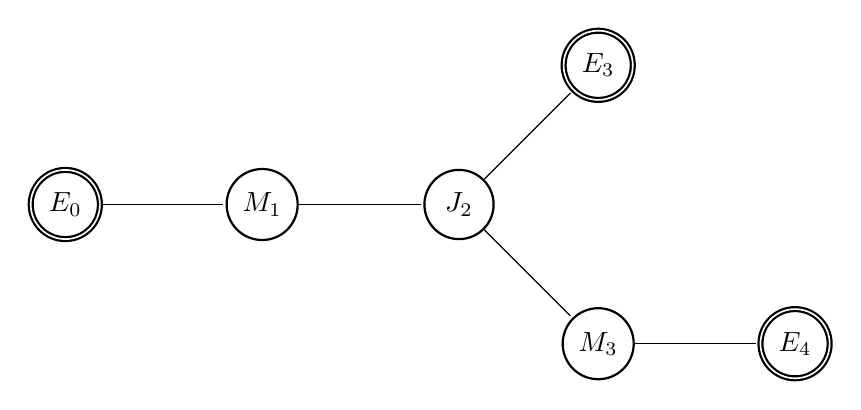
\begin{tikzpicture}[shorten >=1pt,node distance=2.5cm,on grid,auto] 
   \node[state,accepting,thick] (R1)   {$E_0$}; 
   \node[state,thick] (R2) [right=of R1] {$M_1$};
   \node[state,thick] (R3) [right=of R2] {$J_2$};
   \node[state,accepting,thick] (R4) [above right=of R3] {$E_3$};
   \node[state,thick] (R5) [below right=of R3] {$M_3$};
   \node[state,accepting,thick] (R6) [right=of R5] {$E_4$};
   %\only<2>{\node [draw,rectangle,text width=5.5cm] (box) at (2.5,2) {%
    %{\scriptsize The chain identifier of a new beacon is determined by incrementing of one unit the chain id of the closest beacon.}
    %};}
    \path[]
    (R1) edge (R2)
    (R2) edge (R3)
    (R3) edge (R4)
    (R3) edge (R5)
    (R5) edge (R6);
\end{tikzpicture}
\vskip10pt
{\footnotesize \emph{Chain example with nodes labeling and id}}
\end{center}
\note{Describe the structure of the chain and the purpose of the different elements:
\begin{itemize}
  \item \emph{Chain End} state is reached when a robot connects himself to the current end of the chain, becoming
thus the new termination.
In this state, the robot stands still and broadcast information concerning its state, id and chain id to the
neighboring robots.
\item \emph{Chain Member} if more than one \emph{Beacon} but less than two are connected to a \emph{Chain End}.
\item \emph{Chain Junction} if more than two \emph{Beacon} are connected to a \emph{Chain Junction}.
\end{itemize}
}
\end{frame}

\begin{frame}[t,fragile]{\textbf{Controller components}}
\vskip10pt
\begin{Large}
\begin{enumerate}
  \item<2-> Chain beginning
  \vskip7pt
  \item<3-> Chain following
  \vskip7pt
  \item<4-> Chain building
  \vskip7pt
  \item<5-> Chain state updating
\end{enumerate}
\end{Large}
\note{
Test}
\end{frame}

\begin{frame}[t,fragile]{\textbf{Chain beginning}}
\begin{tiny}
%\begin{center}
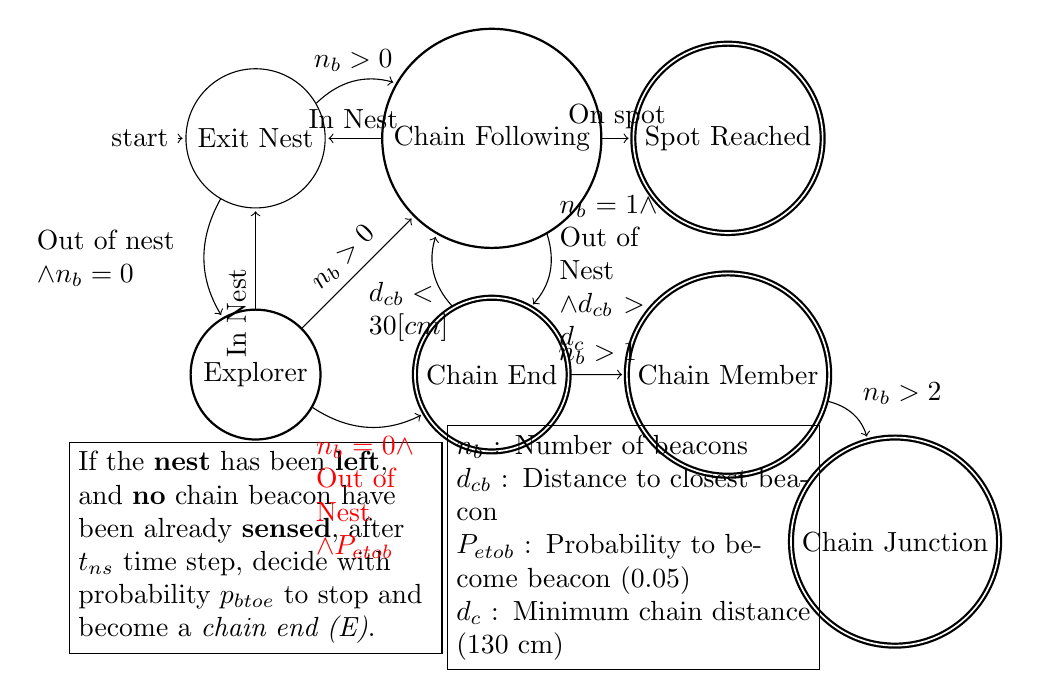
\begin{tikzpicture}[scale=0.2,shorten >=1pt,node distance=3cm,on grid,auto] 
   \node[state,initial] (EN)   {Exit Nest}; 
   \node[state,thick] (EX) [below=of EN] {Explorer};
   \node[state,thick] (EC) [right=of EN] {Chain Following};
   \node[state,accepting,thick] (SR) [right=of EC] {Spot Reached};
   \node[state,accepting,thick] (CE) [below =of EC] {Chain End};
   \node[state,accepting,thick] (CM) [right=of CE] {Chain Member};
   \node[state,accepting,thick] (CJ) [below right=of CM] {Chain Junction};
   \node [draw,rectangle,text width=4.5cm] (box) at (24,-26) {%
    $n_b$ : Number of beacons
     
    $d_{cb}$ : Distance to closest beacon
     
    $P_{etob}$ : Probability to become beacon (0.05)
     
    $d_c$ : Minimum chain distance (130 cm)
    };
    \node [draw,rectangle,text width=4.5cm] (box) at (0,-26) {%
    If the \textbf{nest} has been \textbf{left}, and \textbf{no} chain beacon have been already \textbf{sensed}, after $t_{ns}$ time step, decide with probability $p_{btoe}$ to stop and become a \emph{chain end (E)}.
    };
    \path[->] 
    (EN) edge [bend right]  node [left,text width=2cm]  {Out of nest $\wedge \text{ } n_b = 0$} (EX)
         edge [bend left]  node [above]  {$n_b >0$} (EC)
    (EX) edge node [above,rotate=45]  {$n_b >0$} (EC)
         edge [bend right]  node [red,below,text width=1.3cm]  {$n_b = 0 \text{ } \wedge$ Out of Nest $\wedge \text{ } P_{etob}$} (CE)
          edge  node [above left,rotate=90]  {In Nest} (EN)
    (CE) edge node {$n_b > 1$} (CM)
           edge [bend left] node [below left,text width=0.7cm]  {$d_{cb} < 30[cm]$} (EC)
    (CM) edge [bend left] node [text width=2cm] {$n_b > 2$} (CJ)
    (EC) edge  node [above]  {In Nest} (EN)
           edge [bend left] node [right,text width=1.3cm] {$n_b = 1 \text{ } \wedge$ Out of Nest $\wedge \text{ } d_{cb} > d_c$} (CE)
           edge  node {On spot} (SR);
\end{tikzpicture}
%\captionof{figure}{Implemented FSM for the \emph{s-bot} chain formation behavior}
%\end{center}
\end{tiny}
\note{\begin{scriptsize}
The general idea of the method is that the robots should first quit the initial deployment room, characterized
by four surrounding walls, one of them containing an opening to let the robots move outside, and a dark
grey floor, to then start the exploration phase required to find the target spots.
In order to reduce the interference phenomenon at the exit of the nest, a sequential deployment mechanism
based on the robot id has been developed.
After exiting the nest, the agents should explore the environment, either individually (as explorers) or using
the collectively-gathered knowledge of the environment (i.e. the chain).
If no information is available, the robot could decide (stochastically) to become a starting point for a new
chain in the environment.
Otherwise, the exploration of the environment should, in principle, profit of the already available knowledge.
Nevertheless, this method achieves the required chain formation behavior using the embodied information in
the chain only to exist the nest, while the successive exploration is simply guided by the proximity sensors
and the distance scanner.
\end{scriptsize}
}

\end{frame}


\begin{frame}[t,fragile]{\textbf{Chain following}}
\begin{tiny}
%\begin{center}
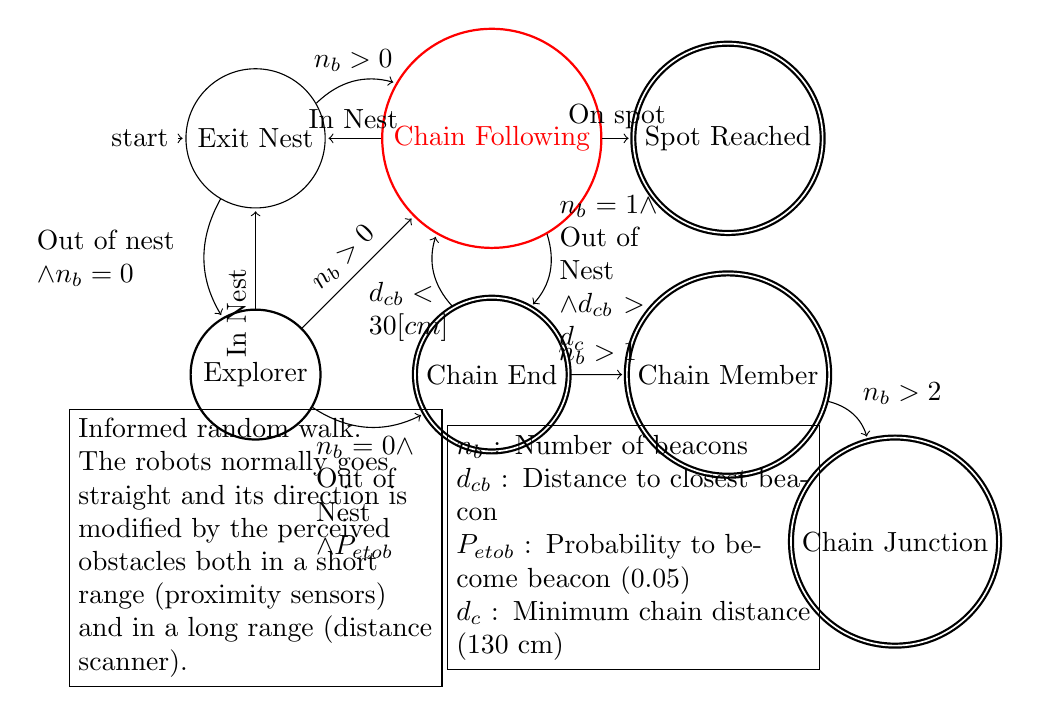
\begin{tikzpicture}[scale=0.2,shorten >=1pt,node distance=3cm,on grid,auto] 
   \node[state,initial] (EN)   {Exit Nest}; 
   \node[state,thick] (EX) [below=of EN] {Explorer};
   \node[state,thick,red] (EC) [right=of EN] {Chain Following};
   \node[state,accepting,thick] (SR) [right=of EC] {Spot Reached};
   \node[state,accepting,thick] (CE) [below =of EC] {Chain End};
   \node[state,accepting,thick] (CM) [right=of CE] {Chain Member};
   \node[state,accepting,thick] (CJ) [below right=of CM] {Chain Junction};
   \node [draw,rectangle,text width=4.5cm] (box) at (24,-26) {%
    $n_b$ : Number of beacons
     
    $d_{cb}$ : Distance to closest beacon
     
    $P_{etob}$ : Probability to become beacon (0.05)
     
    $d_c$ : Minimum chain distance (130 cm)
    };
    \node [draw,rectangle,text width=4.5cm] (box) at (0,-26) {%
    Informed random walk.
    The robots normally goes straight and its direction is modified by the perceived obstacles both in a short range (proximity sensors) and in a long range (distance scanner).
    };
    \path[->] 
    (EN) edge [bend right]  node [left,text width=2cm]  {Out of nest $\wedge \text{ } n_b = 0$} (EX)
         edge [bend left]  node [above]  {$n_b >0$} (EC)
    (EX) edge node [above,rotate=45]  {$n_b >0$} (EC)
         edge [bend right]  node [below,text width=1.3cm]  {$n_b = 0 \text{ } \wedge$ Out of Nest $\wedge \text{ } P_{etob}$} (CE)
          edge  node [above left,rotate=90]  {In Nest} (EN)
    (CE) edge node {$n_b > 1$} (CM)
           edge [bend left] node [below left,text width=0.7cm]  {$d_{cb} < 30[cm]$} (EC)
    (CM) edge [bend left] node [text width=2cm] {$n_b > 2$} (CJ)
    (EC) edge  node [above]  {In Nest} (EN)
           edge [bend left] node [right,text width=1.3cm] {$n_b = 1 \text{ } \wedge$ Out of Nest $\wedge \text{ } d_{cb} > d_c$} (CE)
           edge  node {On spot} (SR);
\end{tikzpicture}
%\captionof{figure}{Implemented FSM for the \emph{s-bot} chain formation behavior}
%\end{center}
\end{tiny}
\end{frame}

\begin{frame}[t,fragile]{\textbf{Chain building}}
\begin{tiny}
%\begin{center}
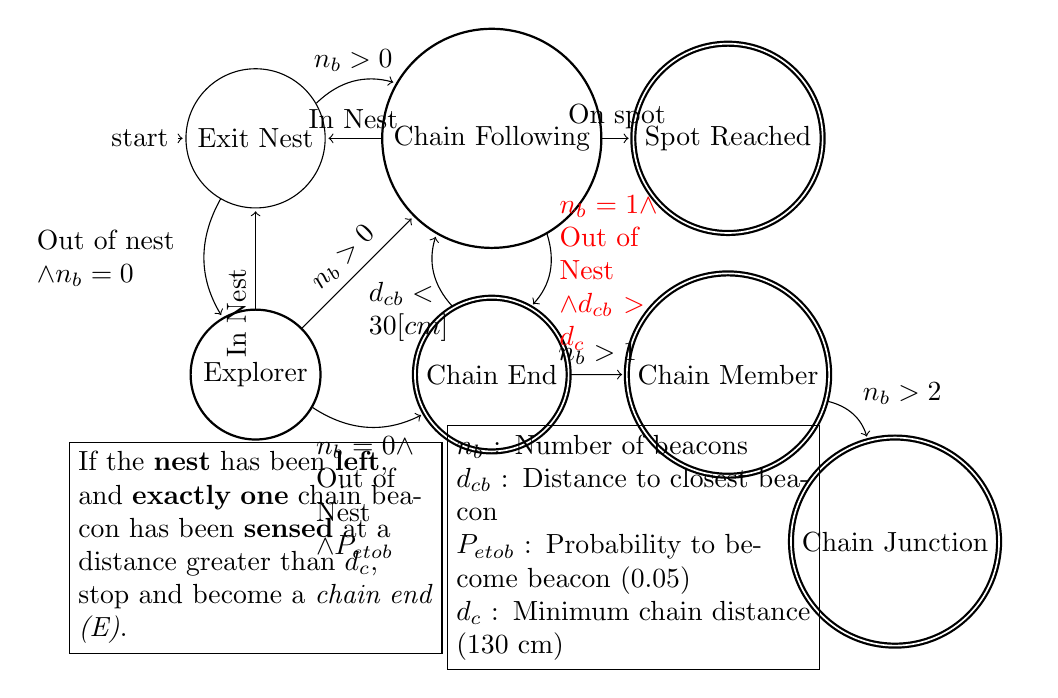
\begin{tikzpicture}[scale=0.2,shorten >=1pt,node distance=3cm,on grid,auto] 
   \node[state,initial] (EN)   {Exit Nest}; 
   \node[state,thick] (EX) [below=of EN] {Explorer};
   \node[state,thick] (EC) [right=of EN] {Chain Following};
   \node[state,accepting,thick] (SR) [right=of EC] {Spot Reached};
   \node[state,accepting,thick] (CE) [below =of EC] {Chain End};
   \node[state,accepting,thick] (CM) [right=of CE] {Chain Member};
   \node[state,accepting,thick] (CJ) [below right=of CM] {Chain Junction};
   \node [draw,rectangle,text width=4.5cm] (box) at (24,-26) {%
    $n_b$ : Number of beacons
     
    $d_{cb}$ : Distance to closest beacon
     
    $P_{etob}$ : Probability to become beacon (0.05)
     
    $d_c$ : Minimum chain distance (130 cm)
    };
    \node [draw,rectangle,text width=4.5cm] (box) at (0,-26) {%
    If the \textbf{nest} has been \textbf{left}, and \textbf{exactly one} chain beacon has been \textbf{sensed} at a distance greater than $d_{c}$, stop and become a \emph{chain end (E)}.
    };
    \path[->] 
    (EN) edge [bend right]  node [left,text width=2cm]  {Out of nest $\wedge \text{ } n_b = 0$} (EX)
         edge [bend left]  node [above]  {$n_b >0$} (EC)
    (EX) edge node [above,rotate=45]  {$n_b >0$} (EC)
         edge [bend right]  node [below,text width=1.3cm]  {$n_b = 0 \text{ } \wedge$ Out of Nest $\wedge \text{ } P_{etob}$} (CE)
          edge  node [above left,rotate=90]  {In Nest} (EN)
    (CE) edge node {$n_b > 1$} (CM)
           edge [bend left] node [below left,text width=0.7cm]  {$d_{cb} < 30[cm]$} (EC)
    (CM) edge [bend left] node [text width=2cm] {$n_b > 2$} (CJ)
    (EC) edge  node [above]  {In Nest} (EN) 
           edge [bend left] node [red,right,text width=1.3cm] {$n_b = 1 \text{ } \wedge$ Out of Nest $\wedge \text{ } d_{cb} > d_c$} (CE)
           edge  node {On spot} (SR);
\end{tikzpicture}
%\captionof{figure}{Implemented FSM for the \emph{s-bot} chain formation behavior}
%\end{center}
\end{tiny}
\end{frame}


\begin{frame}[t,fragile]{\textbf{Chain updating}}
\begin{tiny}
%\begin{center}
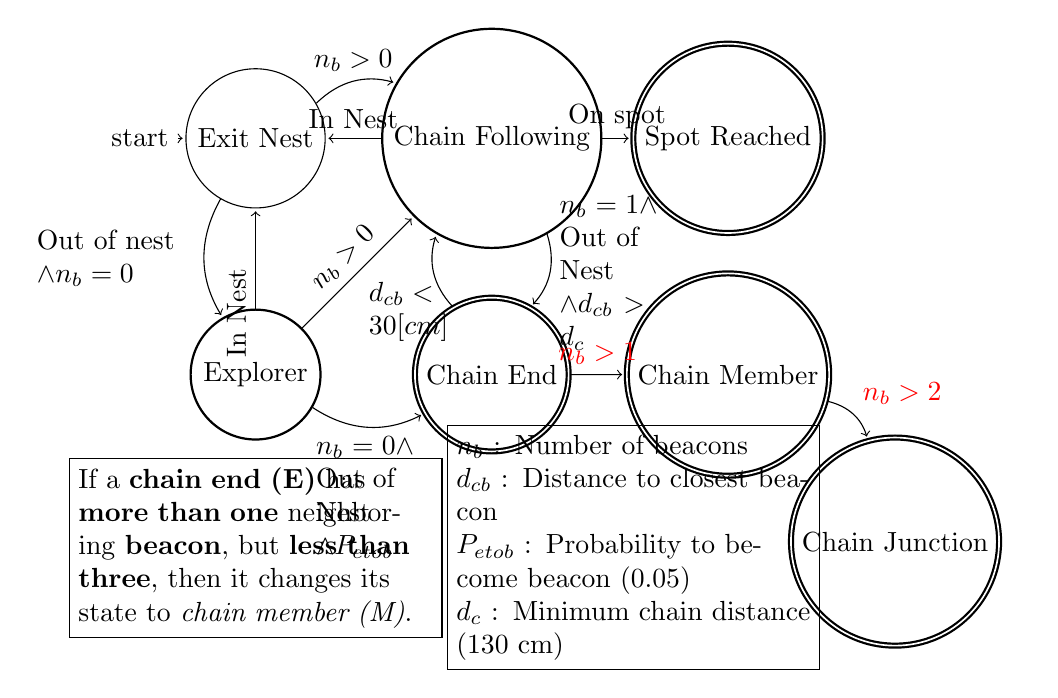
\begin{tikzpicture}[scale=0.2,shorten >=1pt,node distance=3cm,on grid,auto] 
   \node[state,initial] (EN)   {Exit Nest}; 
   \node[state,thick] (EX) [below=of EN] {Explorer};
   \node[state,thick] (EC) [right=of EN] {Chain Following};
   \node[state,accepting,thick] (SR) [right=of EC] {Spot Reached};
   \node[state,accepting,thick] (CE) [below =of EC] {Chain End};
   \node[state,accepting,thick] (CM) [right=of CE] {Chain Member};
   \node[state,accepting,thick] (CJ) [below right=of CM] {Chain Junction};
   \node [draw,rectangle,text width=4.5cm] (box) at (24,-26) {%
    $n_b$ : Number of beacons
     
    $d_{cb}$ : Distance to closest beacon
     
    $P_{etob}$ : Probability to become beacon (0.05)
     
    $d_c$ : Minimum chain distance (130 cm)
    };
    \node [draw,rectangle,text width=4.5cm] (box) at (0,-26) {%
    If a \textbf{chain end (E)} has \textbf{more than one} neighboring\textbf{ beacon}, but \textbf{less than three}, then it changes its state to \emph{chain member (M)}.
    };
    \path[->] 
    (EN) edge [bend right]  node [left,text width=2cm]  {Out of nest $\wedge \text{ } n_b = 0$} (EX)
         edge [bend left]  node [above]  {$n_b >0$} (EC)
    (EX) edge node [above,rotate=45]  {$n_b >0$} (EC)
         edge [bend right]  node [below,text width=1.3cm]  {$n_b = 0 \text{ } \wedge$ Out of Nest $\wedge \text{ } P_{etob}$} (CE)
          edge  node [above left,rotate=90]  {In Nest} (EN)
    (CE) edge node [red] {$n_b > 1$} (CM)
           edge [bend left] node [below left,text width=0.7cm]  {$d_{cb} < 30[cm]$} (EC)
    (CM) edge [bend left] node [text width=2cm,red] {$n_b > 2$} (CJ)
    (EC) edge  node [above]  {In Nest} (EN) 
           edge [bend left] node [right,text width=1.3cm] {$n_b = 1 \text{ } \wedge$ Out of Nest $\wedge \text{ } d_{cb} > d_c$} (CE)
           edge  node {On spot} (SR);
\end{tikzpicture}
%\captionof{figure}{Implemented FSM for the \emph{s-bot} chain formation behavior}
%\end{center}
\end{tiny}
\end{frame}


\section{Results}
\begin{frame}[t,fragile]{\textbf{Completion time}}

\begin{minipage}{.47\textwidth}
\centering
\includegraphics[width=0.9\textwidth,keepaspectratio]{{../Results/50Trials/Panel1}.pdf}

{\scriptsize (a)}
\end{minipage}%
\hspace{0.15cm}
\begin{minipage}{.47\textwidth}
\centering
\includegraphics[width=0.9\textwidth,keepaspectratio]{{../Results/50Trials/Panel2}.pdf}

{\scriptsize (b)}
\end{minipage}
\vfill
\begin{center}
\begin{footnotesize}
\emph{Observed distribution of the experiments' completion times over 50 trials displayed as histogram (a) and empirical cumulative density function (b). 

50 Robots. RAB Range: 150$[cm]$.}
\end{footnotesize}
\end{center}
\note{
\begin{scriptsize}
\begin{center}
\begin{tabular}{|l|c|c|}
\hline
& \multicolumn{1}{p{2cm}|}{\textbf{Robots in Chain}} & \multicolumn{1}{p{2cm}|}{\textbf{Completion Time}} \\
\hline
\textbf{Mean} &	36.82 & 21779.52 \\
\hline
\textbf{Std Dev} & 2.5689671 & 11138.0954867 \\
\hline
 \textbf{CV} = $\frac{\sigma}{\mu}$ & 0.06952743 &	0.51140223 \\
\hline
 \textbf{Median} & 37 &	21209.5 \\
\hline
\textbf{Min} & 30 & 6133 \\
\hline
\textbf{Max} & 41 & 47097 \\
\hline
\end{tabular}
\end{center}
\end{scriptsize}

\begin{footnotesize}
\begin{itemize}
  \item 75\% of the trials completed within 30000 timesteps but high CV.
  \item Influence of random seed on robots' initial position and orientation and stochastic decision to stop of the first robot.
\end{itemize}

\end{footnotesize}

}

\end{frame}


\begin{frame}[t,fragile]{\textbf{Robots in chain}}
\begin{minipage}{.47\textwidth}
\centering
\includegraphics[width=0.9\textwidth,keepaspectratio]{{../Results/50Trials/Panel3}.pdf}

{\scriptsize (a)}
\end{minipage}%
\hspace{0.15cm}
\begin{minipage}{.47\textwidth}
\centering
\includegraphics[width=0.9\textwidth,keepaspectratio]{{../Results/50Trials/Panel4}.pdf}

{\scriptsize (b)}
\end{minipage}
\vfill
\begin{center}
\begin{footnotesize}
\emph{Observed distribution of the number of robots in chain over 50 trials displayed as histogram (a) and empirical cumulative density function (b). 

50 Robots. RAB Range: 150$[cm]$.}
\end{footnotesize}
\end{center}

\note{
\begin{scriptsize}
\begin{center}
\begin{tabular}{|l|c|c|}
\hline
& \multicolumn{1}{p{2cm}|}{\textbf{Robots in Chain}} & \multicolumn{1}{p{2cm}|}{\textbf{Completion Time}} \\
\hline
\textbf{Mean} &	36.82 & 21779.52 \\
\hline
\textbf{Std Dev} & 2.5689671 & 11138.0954867 \\
\hline
 \textbf{CV} = $\frac{\sigma}{\mu}$ & 0.06952743 &	0.51140223 \\
\hline
 \textbf{Median} & 37 &	21209.5 \\
\hline
\textbf{Min} & 30 & 6133 \\
\hline
\textbf{Max} & 41 & 47097 \\
\hline
\end{tabular}
\end{center}
\end{scriptsize}

\begin{footnotesize}
High variability in the number of robots:
\begin{itemize}
  \item Random walk
  \item Distance scanner force tailored for target reachability instead of optimal placement
  \item Landmarks sensed only while being on top of them
  \item Bifurcations of the chain
\end{itemize}

\end{footnotesize}
}


\end{frame}

\begin{frame}[t,fragile]{\textbf{Correlation}}
\begin{center}
\includegraphics[width=.7\textheight,keepaspectratio]{{../Results/50Trials/ResultsDistributionCropped}.pdf}  

\begin{footnotesize}
Scatterplot of the experiments' completion times versus the number of robots in chain on 50 trials. 

50 Robots. RAB Range: 150$[cm]$. $r=0.7934599$.
\end{footnotesize}\end{center}
\note{
\begin{center}
\begin{tabular}{|l|c|c|}
\hline
& \textbf{Value} & \textbf{P-Value} \\
\hline
\textbf{Pearson - } $\mathbf{r}$  &	0.7934599 & 6.357e-12 \\
\hline
\textbf{Kendall -} $\mathbf{\tau}$ & 0.6691023 & 5.554e-11 \\
\hline
\end{tabular}  
\end{center}

Positive and significant correlation between completion times and number of robots in chain.
}
\end{frame}

\section{Conclusions}

\begin{frame}[t,fragile]{\textbf{Conclusions}}
\begin{large}
\begin{itemize}
  \vskip10pt
  \item<1-> Simple method:
  \begin{itemize}
    \item Random walk
    \item Limited communication
  \end{itemize}
  \vskip10pt
  \item<2-> Here, simplicity entails:
  \begin{itemize}
    \item Lack of placement optimality
    \item High results variability
  \end{itemize}
  \vskip10pt
  \item<3-> The width of the communication range impacts on:
  \begin{itemize}
    \item Completion time
    \item Number of robots in chain
  \end{itemize}
  \vskip10pt
  \item<4-> Relevant impact of the structure of the environment on the method's performance.
\end{itemize}
\end{large}

\note{
Communication is only used to:
  \begin{itemize}
    \item Speed up the exit from the nest
    \item Determine the distance from the closest beacon
  \end{itemize}
}
\end{frame}
 

\begin{frame}[t,fragile]{\textbf{Questions ?}}
\begin{center}

\includegraphics[height=.8\textheight,keepaspectratio]{UlbLogos/Questions.jpg}
\end{center}
\end{frame}

% \section{Context of the research}
% \begin{frame}[t,fragile]{Research context}
% The evaluation of interactive segmentation is generally done by means of user experimentation.\newline
% This method is effective, but also labor-intensive and time-consuming.\newline 
% The paper proposes an automated approach imitating human behaviour, evaluating it using 4 different algorithms:
% \begin{enumerate}
% \item \textbf{BPT: }Interactive segmentation using Binary Partition Trees
% \item \textbf{IGC: } Interactive Graph Cuts
% \item \textbf{SRG: } Seeded Region Growing 
% \item \textbf{SIOX: } Simple Interactive Object Extraction
% \end{enumerate}
% These algorithms provide a good coverage of the underlying algorithmic approaches described in the literature for
% object extraction from natural scenes.

% \end{frame}

% \section{Theoretical notions}

% \begin{frame}[t,fragile]{User-based segmentation}
% \begin{center}
% \includegraphics[height=.8\textheight,keepaspectratio]{AutomationSchema}
% \end{center}
% \end{frame}

% \begin{frame}[t,fragile]{Strategies overview}
% \begin{itemize}
% \item \textbf{Strategy 1 -} Deterministic choice of ground truth objects centers as seed points.
% \item \textbf{Strategy 2 -} Non-deterministic choice of seeds points with distance-proportional probability.
% \item \textbf{Strategy 3 -} Computation of the shortest seed line defining an acceptable segmentation.
% \item \textbf{Strategy 4 -} Computation of the shortest seed line defining an acceptable segmentation with preference for those passing near the center of the object.
% \end{itemize}
% \end{frame}

% \begin{frame}[t,fragile]{Automated Strategy 1 - Overview}
% Seed points are chosen in a way that :
% \begin{itemize}
%   \item \textbf{(Initialization) -}Intuitively, points closer to the center of the ground truth object are marked as object point, while points clearly outside of it are marked as background
%   \item \textbf{(Update) -} Update seed points are chosen within large misclassified areas
% \end{itemize}
% \textbf{Strong points :}
% \begin{itemize}
%   \item Efficient computation using fast 2D Euclidian distance. 
%   \item Determinism.
%   \item Useful baseline for comparisons.
% \end{itemize}
% \textbf{Weak points :}
% \begin{itemize}
%   \item Determinism does not allow to test the robustness of the strategy.
%   \item Seeds have the form of pixel blobs instead of curves.
% \end{itemize}
% \end{frame}


% \begin{frame}[t,fragile]{Automated Strategy 2 - Overview}
% The strategy is similar to the previous one, the main difference being a non deterministic choice of the points according to a probability distribution which is proportional
% to the distance of points within the candidate set to points outside this set. \newline
% \textbf{Strong points :}
% \begin{itemize}
%   \item Efficient computation using inversion method to compute the probability.
%   \item Non-Determinism allows to test repeatability, hence robustness.
% \end{itemize}
% \textbf{Weak points :}
% \begin{itemize}
%   \item Seeds have the form of pixel blobs instead of curves.
% \end{itemize}
% \end{frame}

% \begin{frame}[t,fragile]{Automated Strategy 1-2 - Example}
% \begin{center}
% \includegraphics[height=.8\textheight,keepaspectratio]{Strategy1Ex}
% \end{center}
% \end{frame}


% \begin{frame}[t,fragile]{Automated Strategy 3 - Overview}
% The seed set will have the form of an automatically generated line, obtained by applying Dijkstra's shortest path algorithm on the adjacency graph of the candidate pixels.
% The line will be eventually expanded using a brush function to ensure a better coverage of the object.\newline
% \textbf{Strong points :}
% \begin{itemize}
%   \item Efficient computation of connection relationship and shortest path using Dijkstra's algorithm.
%   \item Seed line define a better coverage of the ground truth object than pixel blobs.
% \end{itemize}
% \textbf{Weak points :}
% \begin{itemize}
%   \item Shortest seed line tends to be closer to the border than desired.
% \end{itemize}
% \end{frame}

% \begin{frame}[t,fragile]{Automated Strategy 3 - Example}
% \begin{center}
% \includegraphics[height=.5\textheight,keepaspectratio]{Strategy3Ex}
% \end{center}
% \end{frame}

% \begin{frame}[t,fragile]{Automated Strategy 4 - Overview}
% This strategy is identical to the previous one, except for the weight assigned to each edge in the adjacency graph, which is modified in order to produce
% seed lines which pass closer to the center of the ground truth object.\newline
% \textbf{Strong points :}
% \begin{itemize}
%   \item Efficient computation of connection relationship and shortest path using Dijkstra's algorithm.
%   \item Seed line define a better coverage of the ground truth object than pixel blobs.
% \end{itemize}
% \textbf{Weak points :}
% \begin{itemize}
%   \item Shortest seed line tends to be closer to the border than desired.
% \end{itemize}
% \end{frame}

% \begin{frame}[t,fragile]{Automated Strategy 3 - Example 1}
% \begin{center}
% \includegraphics[height=.5\textheight,keepaspectratio]{Strategy3Ex2}
% \end{center}
% \end{frame}

% \begin{frame}[t,fragile]{Automated Strategy 3 - Example 2}
% \begin{center}
% \includegraphics[height=.7\textheight,keepaspectratio]{Strategy4Ex}
% \end{center}
% \end{frame}

% \section{Results Analysis}
% \begin{frame}[t,fragile]{Evaluation method}
% Given an input image and the corresponding ground truth:
% \begin{enumerate}
% \item Select strategy and algorithm.
% \item Process image according to strategy and algorithm.
% \item Compute object accuracy and border accuracy.
% \item Update seeds.
% \item If maximum step number has been reached stop, else goto 2.
% \end{enumerate}
% \begin{itemize}
%   \item Non deterministic strategy are rerunned 5 times in order to evaluate repeatability.
%   \item The maximum number of steps is equal to 100, which is unrealistic compared to human interaction, to allow stabilization of the results and to observe the strategy behavior over a long run.
%   \item Object and border accuracy will result in a time series of values.
%   \item Accuracy =  $\frac{TruePositive}{TruePositive+FalsePositive+FalseNegative}$ (Jaccard Index)
% \end{itemize}
% \end{frame}

% \begin{frame}[t,fragile]{Evaluation metrics}
% \begin{itemize}
%   \item \textbf{(Profile) - Time-Accuracy Profile } Average accuracy profile across time.
%   \item \textbf{(Aggregate) - Final Accuracy } Accuracy achievable across a reasonable amount of time.
%   \item \textbf{(Aggregate) - Integrated Accuracy } Accuracy integrated over time series data expanded in order to be comparable 
% \end{itemize}
% \begin{itemize}
%   \item These metrics can be averaged across all the object in the dataset to assess overall system performance.
%   \item Integrated accuracy is computed as a discrete summation of the area below the expanded time series.
%   \item Useful because it can be easily normalized with respect to the unity rectangle and briefly express the trend of average accuracy.
%   \item  Must be computed also for user interaction where steps are not unit spaced (i.e resampling or trapezoid rule).
% \end{itemize}
% \end{frame}

% \begin{frame}[t,fragile]{User Interaction Results}
% \begin{center}
% \includegraphics[height=.8\textheight,keepaspectratio]{MeanAccuracyUser}
% \end{center}
% \end{frame}

% \begin{frame}[t,fragile]{Automation Results - Accuracy Profile}
% \begin{center}
% \includegraphics[height=.8\textheight,keepaspectratio]{MeanAccuracyAutomation}
% \end{center}
% \end{frame}

% \begin{frame}[t,fragile]{Automation Results - Final Accuracy}
% \begin{center}
% \includegraphics[height=.7\textheight,keepaspectratio]{MeanAccuracyFinal}
% \end{center}
% \end{frame}

% \begin{frame}[t,fragile]{Automation Results - Integrated Accuracy}
% \begin{center}
% \includegraphics[height=.7\textheight,keepaspectratio]{MeanAccuracyIntegrated}
% \end{center}
% \end{frame}

% \begin{frame}[t,fragile]{Correlation metrics}
% \begin{itemize}
%   \item \textbf{Pearson's product-moment coefficient} 
%   \item \textbf{Spearman's $\rho$ rank coefficient}
% \end{itemize}
% \begin{itemize}
%   \item User (time-based) and automated (step-based) data must be aligned to perform correlation analysis.
%   \item Step-accuracy correlation analysis is limited to 60 step, because of results stabilization and limited number of user interactions.
%   \item Aggregated measures are averaged across different users (for human interaction) or different runs (for non-deterministic strategies) before performing correlation analysis.
%   \item High correlation between user and automated accuracy profile will show that the proposed method is well-emulating human behavior. 
% \end{itemize}
% \end{frame}

% \begin{frame}[t,fragile]{Automation Results - Step-accuracy correlation}
% \begin{center}
% \includegraphics[height=.6\textheight,keepaspectratio]{StepwiseCorrelation}
% \end{center}
% \end{frame}

% \begin{frame}[t,fragile]{Automation Results - Aggregate values correlation}
% \begin{center}
% \includegraphics[height=.7\textheight,keepaspectratio]{AggregateCorrelation}
% \end{center}
% \end{frame}

% \begin{frame}[t,fragile]{Conclusions}
% \begin{itemize}
% \item All the strategies have lead to results which are similar to those obtained with user segmentation.
% \item Strategy 3 and 4 have shown to be the most effective strategies at approximating real user input (highest rank correlation), with strategy 4 time accuracy profile having the closer visual correspondence with respect to user experiments one. 
% \item User evaluation is still the most effective way to evaluate interactive segmentation.
% \item Automated evaluation could provide useful and informative results whenever user test cannot be performed (e.g. due to high time consumption).
% \end{itemize}
% \end{frame}

%\frame{Test}

\begin{frame}[allowframebreaks]
         \frametitle{References}
         \bibliographystyle{alpha}
         \bibliography{References}
\end{frame}


\end{document}
